\documentclass{article}
\usepackage{amsmath, amsthm, amssymb, booktabs, hyperref, graphicx, float, esint, xcolor, subcaption}
\setlength{\abovedisplayskip}{0pt}
\setlength{\belowdisplayskip}{0pt}
\setlength{\abovedisplayshortskip}{0pt}
\setlength{\belowdisplayshortskip}{0pt}

\newcommand{\vr}{\vec{r}}
\newcommand{\vOmega}{\vec{\Omega}}
\newcommand{\vO}{\vec{\Omega}}
\newcommand{\bra}{\left\langle}
\newcommand{\ket}{\right\rangle}
\newcommand{\sbra}{\left[}
\newcommand{\sket}{\right]}
\newcommand{\vdiv}{\vec{\nabla} \cdot}
\newcommand{\vgrad}{\vec{\nabla}}
\newcommand{\vbeta}{\vec{\beta} }
\newcommand{\pdx}{\frac{\partial}{\partial x}}
\newcommand{\pdy}{\frac{\partial}{\partial y}}
\newcommand{\pdz}{\frac{\partial}{\partial z}}
\newcommand{\intrrr}{\int d^3 r \,}
\newcommand{\intrr}{\int d^2 r \,}
\newcommand{\dEdphi}{\partial_\phi E \,}
\newcommand{\dEdp}{\partial_p E \,}
\newcommand{\dBdphi}{\partial_\phi B \,}
\newcommand{\dBdp}{\partial_p B \,}
\newcommand{\adj}{\phi^\dag}
\newcommand{\surf}{\int_{\partial V}}
\newcommand{\bound}{\partial V}
\newcommand{\vn}{\vec{n}}
\newcommand{\Edd}{\mathbf{E}}
\newcommand{\BEdd}{\mathbf{B}}
\newcommand{\sigt}{\sigma_t}
\newcommand{\sigs}{\sigma_s}
\newcommand{\siga}{\sigma_a}
\newcommand{\isigt}{c}
\newcommand{\angSource}{q_\Omega}
\newcommand{\scalSource}{q}
\newcommand{\angResp}{q^\dag}
\newcommand{\scalResp}{q^\dag}
\newcommand{\qoi}{QoI}

\begin{document}
\begin{center}
{\large Thesis Proposal }\\
Ian Halvic, Texas A\&M University, NUEN \\
Adjoint-based sensitivity for radiation transport using an Eddington tensor formulation \\
\end{center}

\tableofcontents

%%%%%%%%%%%%%%%%%%%%%%%%%%%%%%%%%%%%%%%%%%%%%%%%%%%%%%%%%%%%%%%%%%%%%%%%%%%%%%%%%%%%%%%%%%%%%%%%%%%%
\section{Introduction}
%%%%%%%%%%%%%%%%%%%%%%%%%%%%%%%%%%%%%%%%%%%%%%%%%%%%%%%%%%%%%%%%%%%%%%%%%%%%%%%%%%%%%%%%%%%%%%%%%%%%
\begin{itemize}
\item predictive science -> need for UQ and sensitivity [Nat'l Aca]
\item adjoint methods have been dev. to provide sensi coefs; [Marchuk]; mathematical technique based on inner products; why useful: many sources -> many direct solve (forward) but only 1 forward and 1 adjoint for same answers
\item adjoint methods also used for time-dep problems [find refs, fluid flow, Sandia]. in time-dep problem, the forward time-dep solution needs to be stored for later use in the adjoitn formalism [put that proof with a simple linear operator du/dt + Au = q in appendix of thesis]
\item time-dep transport would require very large memory usage to store forward solution because rad transport is a 6D (high dimensional phase space problem at every time step)
\item idea investigated in this these: use of an low-order representation for rad transport: VET. 
\item: setting of the study: single group (one-speed) steady state transport 
\end{itemize}
[IWH: REMOVE ABOVE LIST]

Computational simulations have become important tools for engineers and scientists across a wide array of disciplines. These simulations allow for researchers to examine significantly complex and long life systems in a way that is frequently more economical in both time and money than construction of the real world system, if even feasible. An important step in creating one of these methods is confirmation that the results can be trusted to reasonably approximate the real life scenario. This can be accomplished using three process \cite{NRCVVUQ}
\begin{itemize}
\item Verification - How accurately does the computation solve the underlying equations of the model for the quantities of interest?
\item Validation - How accurately does the model represent reality for the quantities of interest?
\item Uncertainty Quantification (UQ) -  How do the various sources of error and uncertainty feed into uncertainty in the model-based prediction of the quantity of interest?
\end{itemize}

Adjoint methods are particularly useful for UQ. In general, adjoint methods provide a mechanism for propagating uncertainty and error in the system variables to the error in the desired quantity of interest. They accomplish this in a particularly economical way, sometimes requiring only two differential system solves which can then be used for any combination of sources of error, as opposed to performing an independent solve for each individual error scenario.

These adjoint methods have been applied across various complex and time dependent systems, including {\color{red}[IWH: find some examples and add here]}

Application of the adjoint method to time dependent transport can pose a major technical limitation. In general, the adjoint method would require storing six-dimensional data at each time step. When dealing with high resolution in these six dimensions and many time steps, this can potentially require an unreasonable amount of memory for data storage, rendering the method functionally unusable.

A potential solution to the memory requirement for the time dependent transport adjoint formulation is the use of a quasi-diffusion method to reduce the overall dimensionality of the transport equation. The method examined in this paper is termed  as a ''Variable Eddington Tensor" formulation, which utilizes a tensor value to relate the scalar flux to higher order angular flux moments. 
%%%%%%%----------------------------------------------------------------------------------------------
\subsection{Steady-state one-group neutron transport equation}
%%%%%%%----------------------------------------------------------------------------------------------
This paper will focus on a relatively simple transport equation form, the one-group steady state transport equation. Examination of the quasi-diffusion's effectiveness in this simple case may provide insight to advantages and shortcomings when applied to a full time dependent transport equation. The one-group steady state transport equation for a volume $V$ bounded by the surface $\partial V$ is given below.
\begin{equation}
\label{SS1GTE}
\vO \cdot \vgrad \psi(\vr,\vO) + \sigt(\vr) \psi(\vr,\vO) = \frac{1}{4 \pi} \sigs(\vr) \phi(\vr) + q(\vr,\vO) 
\end{equation}
\begin{equation}
\psi(\vr,\vO) = \psi^{\text{inc}}(\vr,\vO) \quad \vr \in \partial V^{-} = \{ \vr \in \partial V, \text{ s.t. }, \vO \cdot \vec{n}(\vr) < 0\}
\end{equation}
The given system variables are the total and scattering cross-sections $\sigt$ and $\sigs$, the particle source term $q$, and the external flux incident on the system given by $\psi^{\text{inc}}$. The unknowns are the angular flux $\psi$ and the scalar flux $\phi$.
%%%%%%%----------------------------------------------------------------------------------------------
%\subsection{Quantity of interest and their sensitivities}
%%%%%%%----------------------------------------------------------------------------------------------

%----------------------------------------------------------------------------------------------
\subsubsection{Quantity of interest, response function, and inner products}
%----------------------------------------------------------------------------------------------
Frequently, the solution to the transport equation is not the sought after value, rather some Quantity of Interest ($\qoi$) which depends on the transport solution. Given $\psi(\vr,\vO)$ the solution of the one-group steady-state transport (Eq.~\eqref{SS1GTE}), a QoI
defined as
\begin{equation}
\qoi =  \int_V dV \int_{4 \pi} d \vO \,  r(\vr, \vO) \psi(\vr, \vO)
\end{equation}
where $ r(\vr, \vO)$ is termed the ''response function" which is used to characterize the meaning of the desired $\qoi$. The response function can take on physically defined forms, such as the cross section of a detector; or it may take a form of a mathematical construct, such as $r(\vr, \vO)=1$ to return the total neutrons present in the system. To avoid confusion with the spacial location vector $\vr$ and for reasons that will become clear later, the response function will frequently be expressed as $q^\dag$.

For the sake of brevity in this paper, particularly for expressing the $\qoi$, two volumetric inner products are defined both using $\bra \bullet , \bullet \ket$ notation. These two inner-products are for use with angular and scalar flux respectively. 
\begin{equation}
\bra \psi , \angResp \ket_{V \times \mathcal{S}_2}  = \int_V dV \int_{4 \pi} d \vO \,  \psi(\vr, \vO)\angResp(\vr, \vO)
\end{equation}

\begin{equation}
\bra \phi(\vr) ,\angResp \ket_V  = \int_V dV \,  \phi(\vr)\angResp(\vr)
\end{equation}
For later use, two additional inner products are also defined as surface integrals over the region boundary $\partial V$. The latter splinting incoming and outgoing surface integrals.

\begin{equation}
\sbra \psi , g \sket_{\bound \times \mathcal{S}_2}  = \int_{\bound} dS \int_{4 \pi} d \vO \, \vO \cdot \vn(\vr) \, f(\vr, \vO)g(\vr, \vO)
\end{equation}
\begin{equation}
\sbra \phi , g \sket_{\pm}   = \int_{\bound} dS \int_{\vO \cdot \vn \gtrless 0} d\vO \,  \vO \cdot \vn(\vr) \, f(\vr, \vO)g(\vr, \vO)
\end{equation}


The inner product subscripts will frequently be dropped when it is unambiguous which one being used, typically indicated by $\psi$ or $\phi$. Therefore, with this notation, the quantity of interest can be compactly expressed as shown below.
\begin{equation}
\label{QoIDef}
\qoi = \bra \psi(\vr,\vO), \angResp(\vr,\vO) \ket = \bra \phi(\vr) , \scalResp(\vr) \ket
\end{equation}

%----------------------------------------------------------------------------------------------
\subsubsection{Sensitivity to Inputs}
%----------------------------------------------------------------------------------------------
A hurdle in utilizing the transport equation numerically to make real world predictions is that none of the system's parameters ($\sigt$, $\sigs$, $q$, and $\psi^{inc}$) are ever known exactly. This error in the system parameters is expected to translate to error in the QoI value


%%%%%%%----------------------------------------------------------------------------------------------
\subsection{Adjoint sensitivity}
%%%%%%%----------------------------------------------------------------------------------------------

Adjoint operators can provide a useful tool for sensitivity calculations. Using inner product notation $\bra \bullet , \bullet \ket$, consider the system of interest $\mathbf{A} \psi = q$. Call this this the forward system, with forward operator $\mathbf{A}$. Consider a test function $\psi^\dag$, the adjoint operator $\mathbf{A^\dag}$ is defined such that $\bra \mathbf{A} \psi, \psi^\dag \ket = \bra \psi, \mathbf{A^\dag} \psi^\dag \ket $. For differential operators, derivation of $\mathbf{A^\dag}$ generally relies on application of the divergence theorem (integration by parts), typically resulting in boundary terms ($BC$). Using the response function of the desired $\qoi$, the adjoint system can be constructed as $\mathbf{A^\dag} \psi^\dag = q^\dag$, leading to an alternate expression of the $\qoi$ using the adjoint solution $\psi^\dag $.
\begin{equation}
\label{genAdjQoI}
\qoi = \bra \psi, r \ket = \bra q , \psi^\dag \ket + BC
\end{equation} 
From the above, it follows that a first order approximation to the change in the quantity of interest based on perturbations to the initial system, including perturbation to the forward operator $\delta \mathbf{A}$ and forward source $\delta q$, can be expressed in the form shown in Eq.~\eqref{genAdjSens} \cite{Marchuk}.
\begin{equation}
\label{genAdjSens}
\delta \qoi \approx \bra \delta q - \delta \mathbf{A} \psi , \psi^\dag \ket 
\end{equation}
The advantage of the above expression for $\delta \qoi$ is that two solves, one for the forward and another for the adjoint, can be used to approximate the sensitivity for a variety $\delta \mathbf{A}$ and $\delta q$.

 
%%%%%%%%%%%%%%%%%%%%%%%%%%%%%%%%%%%%%%%%%%%%%%%%%%%%%%%%%%%%%%%%%%%%%%%%%%%%%%%%%%%%%%%%%%%%%%%%%%%%
\section{Discrete Ordinates (Sn) Transport}
%%%%%%%%%%%%%%%%%%%%%%%%%%%%%%%%%%%%%%%%%%%%%%%%%%%%%%%%%%%%%%%%%%%%%%%%%%%%%%%%%%%%%%%%%%%%%%%%%%%%
A discrete ordinates (Sn) method can be used to solve the one group steady state transport equation (Eq.~\eqref{SS1GTE}). The focus of this method is to discretize the angular variable into discrete directions. Using an angular quadrature with $D$ directions $\vO_d$, the transport equation is solved along each direction:
\begin{equation}
\label{1gTE}
\vO_d \cdot \vgrad \psi_d + \sigt \psi_d = \frac{\sigs}{4 \pi} \phi + \frac{q}{4 \pi} \quad \vr \in V , \forall d\in [1,D]
\end{equation}
%
The scalar flux can be computed from the angular flux as follows
\[
\phi(\vr) \approx \sum_{d=1}^D w_d \psi_d(\vr)
\] 
where $\psi_d(\vr) = \psi(\vr, \vO_d)$ and $w_d$ is a quadrature weight. This leads to a coupled system of $D$ equations of the form shown in Eq.~\eqref{snFwd}, where the system is coupled through the scalar flux terms.
%
\begin{equation}
\label{snFwd}
\vO \cdot \vgrad \psi + \sigt \psi = \frac{\sigs}{4 \pi} \phi + q
\end{equation}
\begin{equation}
\psi(\vr) = \psi^{\text{out}}(\vr) \quad \vr \in \bound , Sn \cdot \vec{n} < 0
\end{equation}

%%%%%%%----------------------------------------------------------------------------------------------
\subsection{Adjoint Sn formulation}
%%%%%%%----------------------------------------------------------------------------------------------
In a fairly straightforward application of the adjoint method previously shown, the adjoint equation which corresponds to the Sn transport formulation with response $\angResp$ is
\begin{equation}
\label{snAdj}
- \vO \cdot \vgrad \psi^\dag + \sigt \psi^\dag = \frac{\sigs}{4 \pi} \phi^\dag + \angResp
\end{equation}
%
\begin{equation}
\psi(\vr)^\dag = \psi^{\dag \text{out}}(\vr) \quad \vr \in \bound , Sn \cdot \vec{n} > 0
\end{equation}
where the definition of the adjoint scalar flux $\phi^\dag$ is analogous to the forward definition. It is worth noting that the Sn adjoint equation is in the form of a transport equation, only with the direction of travel reversed ($\vO \to -\vO)$. This often allows for forward Sn transport solvers to be easily adapted to solving the Sn adjoint system. Once the adjoint solution is obtained, the corresponding QoI can be calculated with a simple inner product with the forward source term, as follows from equation \ref{adjGeneral2}. 
%
\begin{equation}
\label{snAdjQoI}
QoI = \bra \psi^\dag , \angSource \ket - \sbra \psi^\dag,  \psi \sket
\end{equation}
%
The surface interval in \ref{snAdjQoI} can be split into incoming and outgoing flux integrals, which are handled by the forward and adjoint boundary conditions respectively. 
%
\begin{equation}
QoI = \bra \psi^\dag , q \ket - \sbra \psi^{\dag \text{out}},  \psi \sket_+ - \sbra \psi^\dag,  \psi^{\text{inc}} \sket_-
\end{equation}

%%%%%%%----------------------------------------------------------------------------------------------
\subsection{Sn Transport Adjoint Sensitivity}
%%%%%%%----------------------------------------------------------------------------------------------

Now consider perturbations to our system. Specifically perturbations of $\delta \sigt$, $\delta \sigs$, and $\delta q$ to the total cross section, scattering cross section and angular source term respectively. In addition, the incident angular flux is also perturbed by $delta \psi^{inc}$. These perturbations result is a perturbed solution to the Sn-transport equation $\psi_p$. Using this $\delta$ notation, the perturbed Sn-equation is shown below
\begin{equation}
\label{snFwdPert}
\vO \cdot \vgrad \psi_p + \sigt \psi_p = \frac{\sigs}{4 \pi} \phi+p + q+p
\end{equation}
\begin{equation}
\psi_p(\vr) = \psi+p^{\text{out}}(\vr) \quad \vr \in \bound , Sn \cdot \vec{n} < 0
\end{equation}
This perturbation may result in a change to the QoI, now given by $\qoi_p=\bra \psi_p , \angResp \ket$. Retaining the unperturbed adjoint equation given in \ref{snAdj} and using a first order approximation of the perturbed Sn transport equation \ref{snPert}, the perturbed QoI can be represented as an inner product not dependent on the perturbed forward solution.
\begin{equation}
\label{snSens}
\begin{split}
QoI_p &=\bra \psi_p , \angResp \ket \\
&=\bra \psi_p , - \vO \cdot \vgrad \psi^\dag + \sigt \psi^\dag - \frac{\sigs}{4 \pi} \phi^\dag  \ket \\
&= \bra  \vO \cdot \vgrad \psi_p + \sigt \psi_p - \frac{\sigs}{4 \pi} \phi_p , \psi^\dag  \ket - \sbra \psi_p, \psi^\dag \sket\\
&= \bra  \scalSource - \delta \sigt \psi + \frac{\delta\sigs}{4 \pi} \phi + \delta \scalSource , \psi^\dag  \ket - \sbra \psi_p, \psi^\dag \sket\\
\end{split}
\end{equation}
Subtraction of the unperturbed $QoI$ expression in equation \ref{snAdjQoI} supplies a final equation for computing the change in $QoI$ using only the system perturbations and the unperturbed forward and adjoint solutions, removing the need to solve the perturbed forward equation.
\begin{equation}
\delta QoI_p = \bra - \delta \sigt \psi + \frac{\delta\sigs}{4 \pi} \phi + \delta \scalSource , \psi^\dag  \ket - \sbra \psi_p, \psi^\dag \sket\\
\end{equation}

%%%%%%%%%%%%%%%%%%%%%%%%%%%%%%%%%%%%%%%%%%%%%%%%%%%%%%%%%%%%%%%%%%%%%%%%%%%%%%%%%%%%%%%%%%%%%%%%%%%%
\section{VET formulation}
%%%%%%%%%%%%%%%%%%%%%%%%%%%%%%%%%%%%%%%%%%%%%%%%%%%%%%%%%%%%%%%%%%%%%%%%%%%%%%%%%%%%%%%%%%%%%%%%%%%%

%%%%%%%----------------------------------------------------------------------------------------------
\subsection{Motivation} 
%%%%%%%----------------------------------------------------------------------------------------------

While the Sn adjoint sensitivity formulation given by \ref{snSens} provides a first-order accurate method to determine the sensitivity to multiple perturbation scenarios using only a single forward and adjoint transport solve, it can quickly run into technical limitations. Specifically for even a one-group time independent system, all solutions to the forward and adjoint system in space and angle must be stored for retrieval later. For a spatially 3-dimensional system, this translates to storing discretized data across 5-dimensions.


%%%%%%%----------------------------------------------------------------------------------------------
\subsection{VET Formulation}
%%%%%%%----------------------------------------------------------------------------------------------

The "Variable Eddington Tensor" (VET) formulation shows promise of reducing the memory requirements when using the adjoint method for sensitivity. To begin the formulation, the steady state transport equation is expanded to the scalar and first angular moment by application of the $\int d \Omega$ and $\int d \Omega \, \vO$ operators to equation \ref{1gTE}, respectively. Using the notation
\begin{equation}
\phi=\int d\Omega \, \psi( \vO )
,\quad
\vec{J}= \int d\Omega \, \vO \psi( \vO )
\end{equation}
the zero-th and first angular moment transport equations are
\begin{equation}
\label{0am}
\vdiv \vec{J} + \sigt \phi = \sigs \phi + \scalSource
\end{equation}
\begin{equation}
\label{1am}
\vdiv \left(  \int d\Omega \vO \vO \psi \right) + \sigt \vec{J} =0 
\end{equation}
The Eddington Tensor $\Edd$ is then introduced as a simplifying approximation relating the second angular moment term in equation \ref{1am} to the scalar flux. 
\begin{equation}
\label{EddDef}
\Edd=\frac{\int d\Omega \vO \vO \psi}{\phi}
\end{equation}
The inclusion of the Eddington tensor allow equation \ref{1am} to be expressed as $\sigt \vec{J} = - \vdiv \Edd \phi$. Using this as a definition of $\vec{J}$ allows us to convert \ref{0am} to the form shown in \ref{VEFForm}, which only has the scalar flux as an unknown. The substitution $\siga = \sigt-\sigs$ was used.
\begin{equation}
\label{VEFForm}
- \vdiv \left( \frac{1}{\sigt}\vdiv \Edd \phi \right) + \siga \phi = \scalSource
\end{equation}
The known incident flux can be used to generate a suitable boundary condition using a "Boundary Eddington Factor" $B$ \cite{Miften}.
\begin{equation}
\frac{1}{\sigma_{t} } \vec{\nabla} \cdot \left(\Edd \phi \right)  = - 2J^- - B \phi \quad \vr \in \bound
\end{equation}
\begin{equation}
B= \frac{\int_{4 \pi} d\Omega \, \left| \Omega_i n_i \right | \psi}{\int_{4\pi} d\Omega \, \psi} \quad \vr \in \bound
\end{equation}

%%%%%%%----------------------------------------------------------------------------------------------
\subsection{Adjoint VET formulation}
%%%%%%%----------------------------------------------------------------------------------------------

The VET formulation necessitates a reformulation of our adjoint. As shown in \ref{adjForm}, the double divergence term present in the forward equation contributes to a double gradient term in the adjoint equation.
\begin{equation}
\label{adjForm}
- \Edd : \left( \vgrad \left( \frac{1}{\sigt}\vgrad \phi^\dag \right) \right) + \siga \phi^\dag = \scalResp
\end{equation}
For reasons that will become apparent during sensitivity calculations, the boundary condition chosen for the adjoint equation is given in \ref{adjVETBC}. Unlike for Sn formulation, the VET adjoint equation does not take the form of a VET transport equation.
\begin{equation}
\label{adjVETBC}
\Edd \cdot \frac{1}{\sigma_{t} } \vec{\nabla} \phi^\dag  = - 2J^{\dag +} - B \phi^\dag \quad \vr \in \Gamma
\end{equation}
To obtain the QoI using this formulation, begin with the typical QoI definition, relocate operators to the forward to substitute the forward source, and apply boundary conditions.
\begin{equation}
\label{VETQoIAdjUnpDeriv}
\begin{split}
QoI=&\bra \phi , \scalResp \ket \\
=&\bra \phi , - \Edd : \left( \vgrad \isigt \vgrad \phi^\dag \right) + \siga \phi^\dag \ket \\
=& \bra - \vdiv \isigt \vdiv \left( \Edd \phi \right) + \siga \phi, \phi^\dag \ket 
- \sbra \phi, \Edd \cdot \isigt \vgrad \phi^\dag \sket  
+ \sbra \phi^\dag, \isigt \vgrad \Edd \phi \sket \\
=&\bra \scalSource , \phi^\dag \ket 
- \sbra \phi , - 2J^{\dag +} - B \phi^\dag \sket + \sbra \phi^\dag, - 2J^- - B \phi  \sket
\end{split}
\end{equation}
The boundary Eddington terms negate and yield a relatively compact form for the QoI
\begin{equation}
\label{VETQoIAdj}
QoI=\bra \scalSource , \phi^\dag \ket 
+ \sbra 2\phi, J^{\dag +} \sket  - \sbra 2\phi^\dag, J^- \sket
\end{equation}

%%%%%%%----------------------------------------------------------------------------------------------
\subsection{VET adjoint sensitivity}
%%%%%%%----------------------------------------------------------------------------------------------

As was done in the Sn transport formulation, once again consider perturbations to the system parameters. However, in contrast to the Sn case, the assumption is also made that the Eddington factor remains unperturbed under these system perturbations. For brevity, the substitution of $\isigt = \sigt^{-1}$ was also made.
\begin{equation}
\label{VEFPert}
- \vdiv \left((\isigt + \delta \isigt)\vdiv \Edd \phi_p \right) + (\siga + \delta \siga)\phi_p = \scalSource + \delta \scalSource
\end{equation}
\begin{equation}
(\isigt + \delta \isigt) \vec{\nabla} \cdot \left(\Edd \phi_p \right)  = - 2J_p^- - B \phi_p \quad \vr \in \bound
\end{equation}
The usual adjoint process is performed, starting with the QoI definition using the perturbed solution and response. 
\begin{equation}
\label{VETSensDeriv}
\begin{split}
\qoi=&\bra \phi_p , \scalResp \ket \\
=&\bra \phi_p , - \Edd : \left( \vgrad \isigt \vgrad \phi^\dag \right) + \siga \phi^\dag \ket \\
=& \bra - \vdiv \isigt \vdiv \left( \Edd \phi_p \right) + \siga \phi_p, \phi^\dag \ket 
- \int_\Gamma d^2 r \, \phi_p \left( \Edd \cdot \isigt \vgrad \phi^\dag \right) \cdot \vec{n}  \\ 
&+ \int_\Gamma d^2 r \, \phi^\dag \left(  \isigt \vgrad \Edd \phi_p \right) \cdot \vec{n} \\
\end{split}
\end{equation}
A first order perturbation approximation of equation \ref{VEFPert} can be used to substitute into the sensitivity equation \ref{VETSensDeriv}, yielding a form independ of the perturbed forward solution.
\begin{equation}
\label{QoIVETAdjNoBC}
\begin{split}
\qoi =& \bra \scalSource + \delta \scalSource + \vdiv \delta \isigt \vdiv \left( \Edd \phi \right) - \delta \siga \phi, \phi^\dag \ket - \sbra \phi_p, \Edd \cdot \isigt \vgrad \phi^\dag \sket + \sbra \phi^\dag, \isigt \vdiv \Edd \phi_p \sket 
\end{split}
\end{equation}
The first surface term can be dealt with readily using the adjoint boundary condition. For the second surface term, a first order approximation of the perturbed forward boundary condition is used for substitution.
\begin{equation}
\label{QoIVETAdj}
\begin{split}
\qoi =& \bra \scalSource + \delta \scalSource + \vdiv \delta \isigt \vdiv \left( \Edd \phi \right) - \delta \siga \phi, \phi^\dag \ket - \int_\Gamma d^2 r \, \phi_p \left( - 2J^{\dag +} - B \phi^\dag \right) \cdot \vec{n} 
\\ &+ \int_\Gamma d^2 r \, \phi^\dag \left( - 2J_p^- - B \phi_p - \delta \isigt \vdiv \Edd \phi \right) \cdot \vec{n} 
\end{split}
\end{equation}
Subtract the adjoint $\qoi$ formulation from equation \ref{VETQoIAdj} to obtain the sensitivity expression for the adjoint VET formulation.
\begin{equation}
\label{SensVETAdjNoBC}
\begin{split}
\delta \qoi =& \bra \delta \scalSource + \vdiv \delta \isigt \vdiv \left( \Edd \phi \right) - \delta \siga \phi, \phi^\dag \ket + \sbra 2\delta \phi, J^{\dag +} \sket  - \sbra 2\phi^\dag, \delta J^- \sket
\\ &- \sbra \phi^\dag, \delta \isigt \vdiv \Edd \phi \sket
\end{split}
\end{equation}


%%%%%%%----------------------------------------------------------------------------------------------
\subsection{Error from unperturbed Eddington assumption}
%%%%%%%----------------------------------------------------------------------------------------------

Beyond the first order approximation common to adjoint formulations, the VET sensitivity formulation also made the assumption that the Eddington tensor remained unperturbed under perturbations of the other parameters. To observe the terms that were dropped in this approximation, consider a reformulation of the perturbed forward equation, this time introducing $\delta \Edd$ and $\delta  B$ terms. 
\begin{equation}
\label{VEFPerEdd}
- \vdiv \left((\isigt + \delta \isigt)\vdiv (\Edd + \delta \Edd) \phi_p \right) + (\siga + \delta \siga)\phi_p = \scalSource + \delta \scalSource
\end{equation}
\begin{equation}
(\isigt + \delta \isigt) \vec{\nabla} \cdot \left((\Edd + \delta \Edd) \phi_p \right)  = - 2J_p^- - (\BEdd +\delta \BEdd) \phi_p \quad \vr \in \Gamma
\end{equation}
The above can be substituted into equation \ref{VETSensDeriv} to yield an expanded $\qoi$ equation, including the Eddington perturbation terms
\begin{equation}
\label{QoIVETAdjNoBCEdd}
\begin{split}
\qoi =& \bra \scalSource + \delta \scalSource + \vdiv \delta \isigt \vdiv \left( \Edd \phi \right) + \vdiv \isigt \vdiv \left( \delta \Edd \phi \right) - \delta \siga \phi, \phi^\dag \ket \\
&- \sbra \phi_p, \Edd \cdot \isigt \vgrad \phi^\dag \sket 
+ \sbra \phi^\dag , \isigt \vdiv \Edd \phi_p \sket
\end{split}
\end{equation}
The boundary condition for the perturbed forward solution takes on a slightly more complex form, as the additional $\delta \Edd$ and $\delta \BEdd$ terms come into play, but the derivation of the sensitivity proceeds similarly to the case ignoring Eddington perturbations.
\begin{equation}
\label{QoIVETAdjEdd}
\begin{split}
\delta \qoi =& \bra \delta \scalSource + \vdiv \delta \isigt \vdiv \left( \Edd \phi \right) + \vdiv \isigt \vdiv \left( \delta \Edd \phi \right) - \delta \siga \phi, \phi^\dag \ket \\
&+ \sbra 2\delta \phi, J^{\dag +} \sket  - \sbra 2\phi^\dag, \delta J^- \sket
- \sbra \phi^\dag, \delta \isigt \vdiv \Edd \phi \sket
\\
&- \sbra  \phi^\dag ,\isigt \vdiv \delta \Edd \phi \sket
- \sbra \phi^\dag, \phi \delta \BEdd \sket
\end{split}
\end{equation} 
Comparing the above formulation with the unperturbed Eddington case shows that the terms lost by the Unperturbed Eddington assumption are 
\begin{equation}
\label{EddErr}
 \bra \vdiv \isigt \vdiv \left( \delta \Edd \phi \right), \phi^\dag \ket
- \sbra  \phi^\dag ,\isigt \vdiv \delta \Edd \phi \sket
- \sbra \phi^\dag, \phi \delta \BEdd \sket
\end{equation} 

%%%%%%%%%%%%%%%%%%%%%%%%%%%%%%%%%%%%%%%%%%%%%%%%%%%%%%%%%%%%%%%%%%%%%%%%%%%%%%%%%%%%%%%%%%%%%%%%%%%%
\section{Preliminary results}
%%%%%%%%%%%%%%%%%%%%%%%%%%%%%%%%%%%%%%%%%%%%%%%%%%%%%%%%%%%%%%%%%%%%%%%%%%%%%%%%%%%%%%%%%%%%%%%%%%%%

At this point, four separate methods for $\qoi$ calculation have been discussed; forward and adjoint inner products for both Sn and VET formulations. When dealing with sensitivity measurements, the forward solutions are expected to give the most exact answer simply because it involves an additional forward solve of the perturbed system for each perturbation case. THe adjoint methods for sensitivity are relying on a first order approximation, however they only require a single forward solve and a single adjoint for use with all perturbation cases. 

The four methods were implemented in a MATLAB finite element method (FEM) solver. Simple one-dimensional test  cases were run, varying which parameter experienced perturbation and the magnitude of the perturbation. The results of the four different sensitivity methods were analyzed to identify cases where the efficient VET adjoint showed promise as a time and memory efficient method for computing sensitivity.
%%%%%%%----------------------------------------------------------------------------------------------
\subsection{Homogeneous initial system, Uniform Perturbations}
%%%%%%%----------------------------------------------------------------------------------------------
The first test case consisted of a 1D homogeneous system, with a volumetric source throughout. Solutions were obtained using a 200 element FEM mesh. Three systems of varying initial cross sections $\sigt$ and $\sigs$ were tested. Perturbations in $\sigt$, $\sigs$, and $\scalSource$ to the system were made uniformly, resulting in the perturbed system remaining homogeneous.

\begin{figure}[H]
\label{HomoPertt}
\centering
\begin{subfigure}{.5\textwidth}
  \centering
  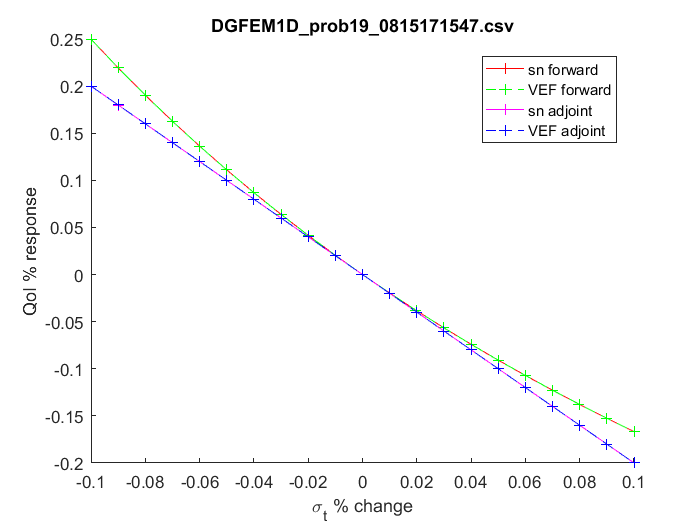
\includegraphics[width=.8\linewidth]{figures/19sigtSens.png}
  \caption{$\sigt=2$, $\sigs=1$}
  \label{fig:sfig1}
\end{subfigure}%
\begin{subfigure}{.5\textwidth}
  \centering
  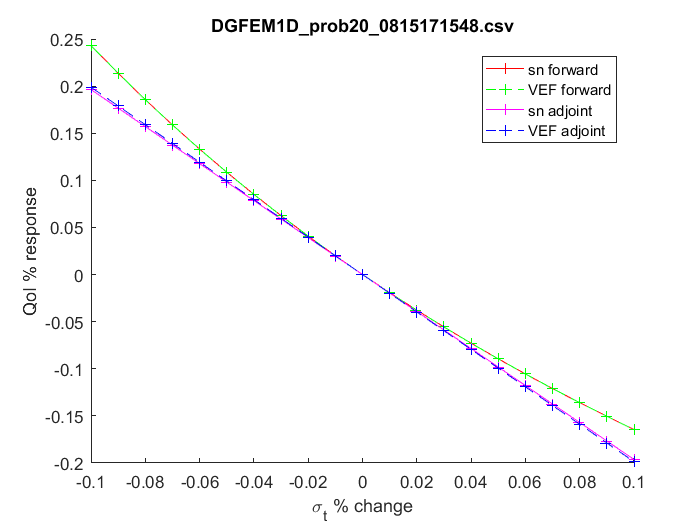
\includegraphics[width=.8\linewidth]{figures/20sigtSens.png}
  \caption{$\sigt=1$, $\sigs=0.5$}
  \label{fig:sfig2}
\end{subfigure}
\begin{subfigure}{.5\textwidth}
  \centering
  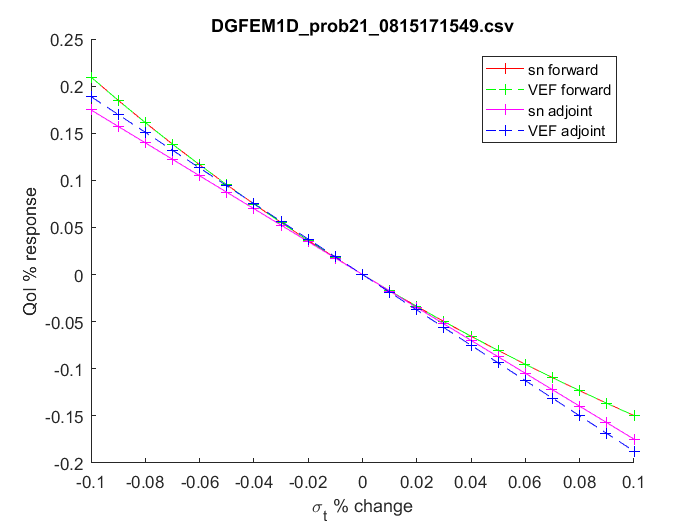
\includegraphics[width=.8\linewidth]{figures/21sigtSens.png}
  \caption{$\sigt=0.5$, $\sigs=0.25$}
  \label{fig:sfig3}
\end{subfigure}
\caption{Plots of $\sigt$ perturbation sensitivity.}
\label{fig:fig}
\end{figure}

\begin{figure}[H]
\label{HomoPerts}
\centering
\begin{subfigure}{.5\textwidth}
  \centering
  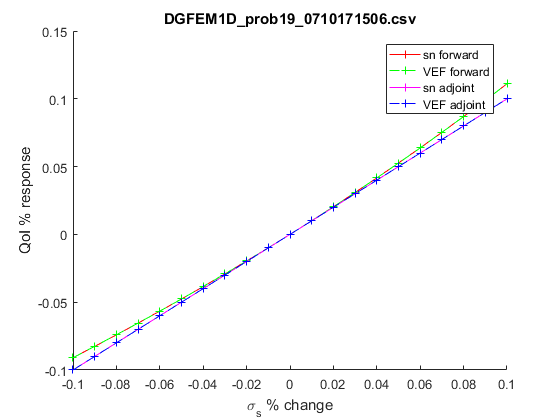
\includegraphics[width=.8\linewidth]{figures/19sigsSens.png}
  \caption{$\sigt=2$, $\sigs=1$}
  \label{fig:sfig1}
\end{subfigure}%
\begin{subfigure}{.5\textwidth}
  \centering
  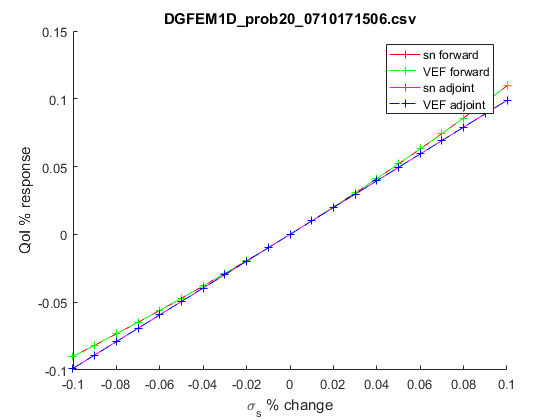
\includegraphics[width=.8\linewidth]{figures/20sigsSens.png}
  \caption{$\sigt=1$, $\sigs=0.5$}
  \label{fig:sfig2}
\end{subfigure}
\begin{subfigure}{.5\textwidth}
  \centering
  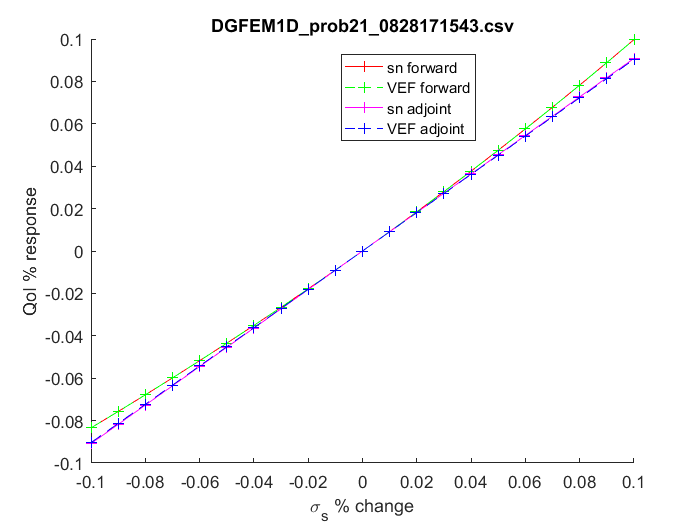
\includegraphics[width=.8\linewidth]{figures/21sigsSens.png}
  \caption{$\sigt=0.5$, $\sigs=0.25$}
  \label{fig:sfig3}
\end{subfigure}
\caption{Plots of $\sigs$ perturbation sensitivity.}
\label{fig:fig}
\end{figure}

\begin{figure}[H]
\label{HomoPertq}
\centering
\begin{subfigure}{.5\textwidth}
  \centering
  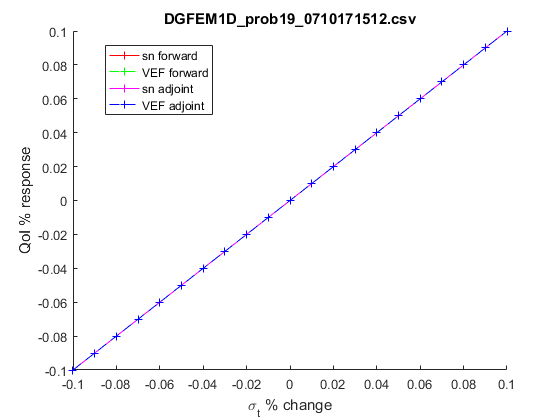
\includegraphics[width=.8\linewidth]{figures/19qSens.png}
  \caption{$\sigt=2$, $\sigs=1$}
  \label{fig:sfig1}
\end{subfigure}%
\begin{subfigure}{.5\textwidth}
  \centering
  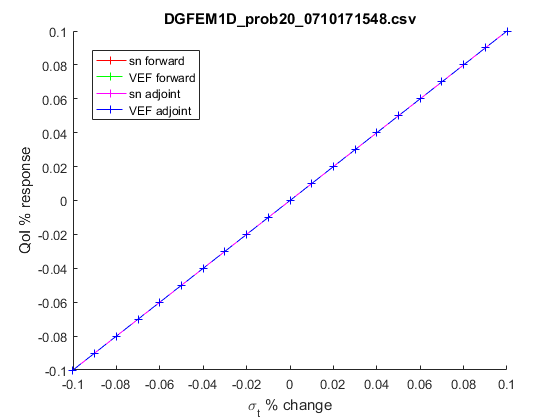
\includegraphics[width=.8\linewidth]{figures/20qSens.png}
  \caption{$\sigt=1$, $\sigs=0.5$}
  \label{fig:sfig2}
\end{subfigure}
\begin{subfigure}{.5\textwidth}
  \centering
  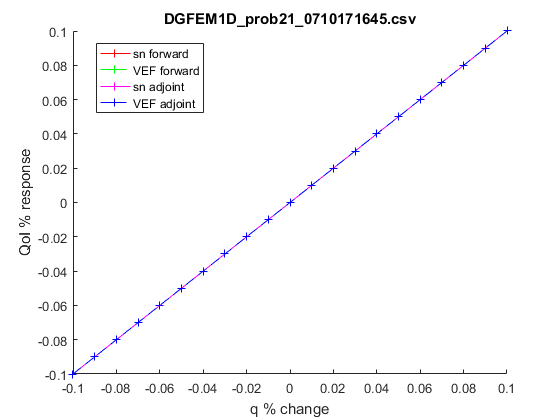
\includegraphics[width=.8\linewidth]{figures/21qSens.png}
  \caption{$\sigt=0.5$, $\sigs=0.25$}
  \label{fig:sfig3}
\end{subfigure}
\caption{Plots of source perturbation sensitivity.}
\label{fig:fig}
\end{figure}

%%%%%%%----------------------------------------------------------------------------------------------
\subsection{Homogeneous initial system, Non-Uniform Perturbations}
%%%%%%%----------------------------------------------------------------------------------------------

[Define system,  perturbations, and QoI. Vary MFP between cases.]
\begin{figure}[H]
\label{InHomoPertt}
\centering
\begin{subfigure}{.5\textwidth}
  \centering
  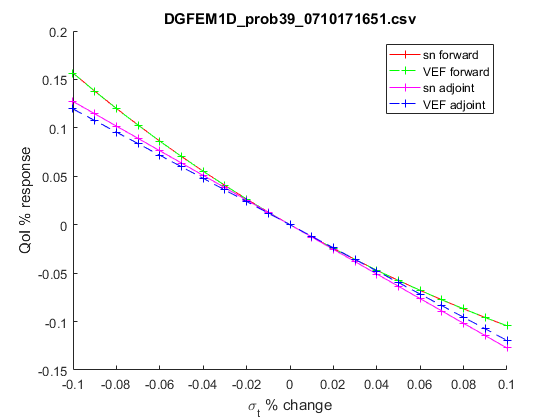
\includegraphics[width=.8\linewidth]{figures/39sigtSens.png}
  \caption{$\sigt=2$, $\sigs=1$}
  \label{fig:sfig1}
\end{subfigure}%
\begin{subfigure}{.5\textwidth}
  \centering
  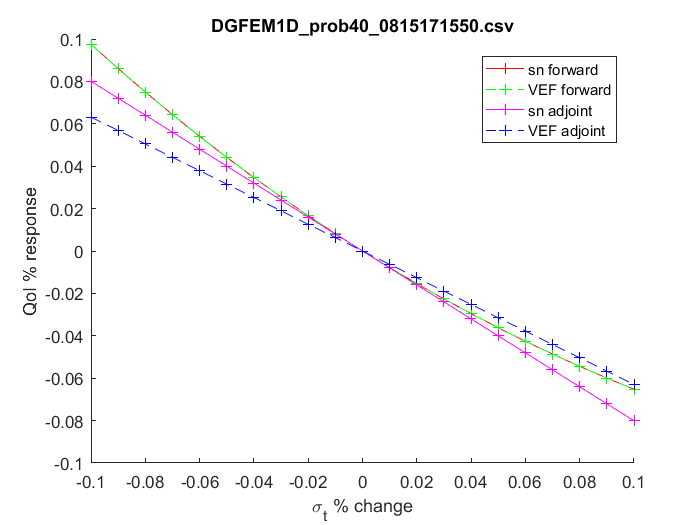
\includegraphics[width=.8\linewidth]{figures/40sigtSens.png}
  \caption{$\sigt=1$, $\sigs=0.5$}
  \label{fig:sfig2}
\end{subfigure}
\begin{subfigure}{.5\textwidth}
  \centering
  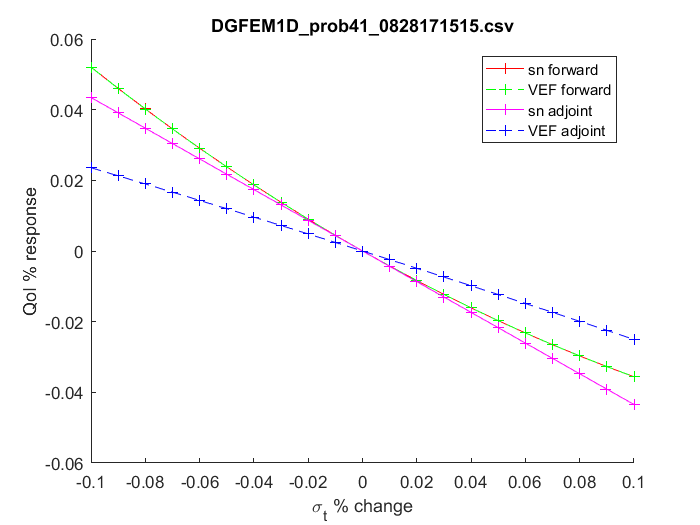
\includegraphics[width=.8\linewidth]{figures/41sigtSens.png}
  \caption{$\sigt=0.5$, $\sigs=0.25$}
  \label{fig:sfig3}
\end{subfigure}
\caption{Plots of $\sigt$ perturbation sensitivity.}
\label{fig:fig}
\end{figure}

\begin{figure}[H]
\label{InHomoPerts}
\centering
\begin{subfigure}{.5\textwidth}
  \centering
  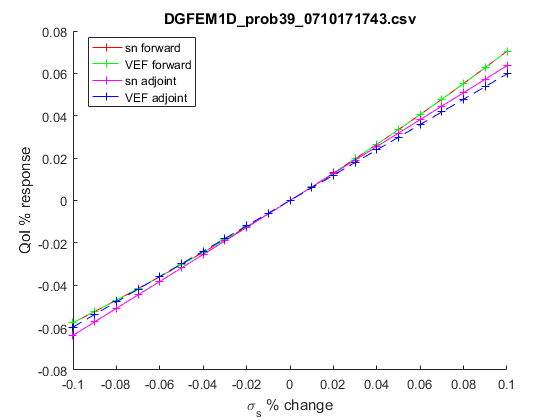
\includegraphics[width=.8\linewidth]{figures/39sigsSens.png}
  \caption{$\sigt=2$, $\sigs=1$}
  \label{fig:sfig1}
\end{subfigure}%
\begin{subfigure}{.5\textwidth}
  \centering
  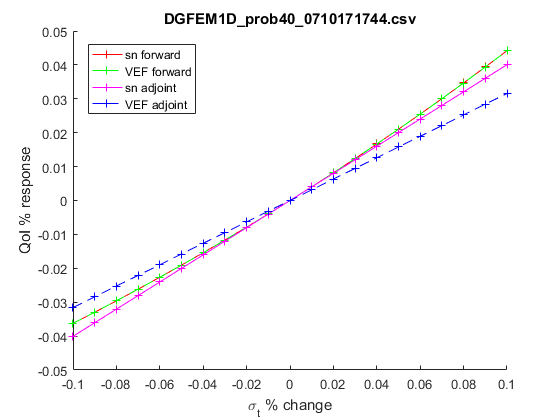
\includegraphics[width=.8\linewidth]{figures/40sigsSens.png}
  \caption{$\sigt=1$, $\sigs=0.5$}
  \label{fig:sfig2}
\end{subfigure}
\begin{subfigure}{.5\textwidth}
  \centering
  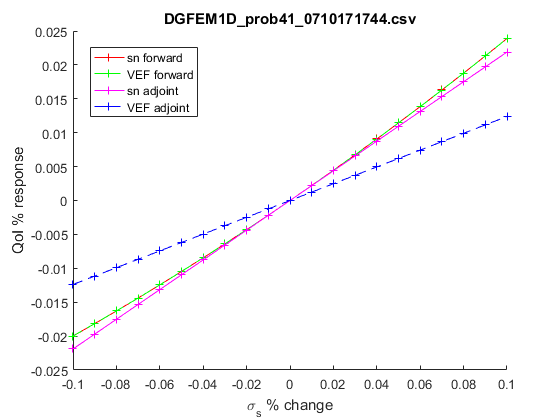
\includegraphics[width=.8\linewidth]{figures/41sigsSens.png}
  \caption{$\sigt=0.5$, $\sigs=0.25$}
  \label{fig:sfig3}
\end{subfigure}
\caption{Plots of $\sigs$ perturbation sensitivity.}
\label{fig:fig}
\end{figure}

\begin{figure}[H]
\label{InHomoPertq}
\centering
\begin{subfigure}{.5\textwidth}
  \centering
  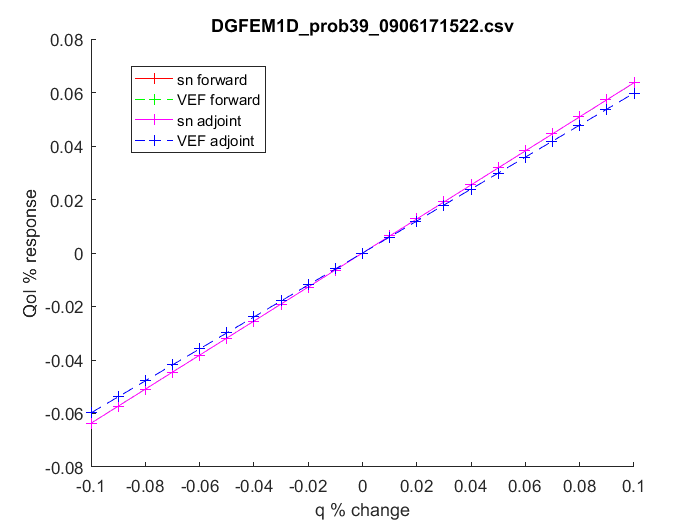
\includegraphics[width=.8\linewidth]{figures/39qSens.png}
  \caption{$\sigt=2$, $\sigs=1$}
  \label{fig:sfig1}
\end{subfigure}%
\begin{subfigure}{.5\textwidth}
  \centering
  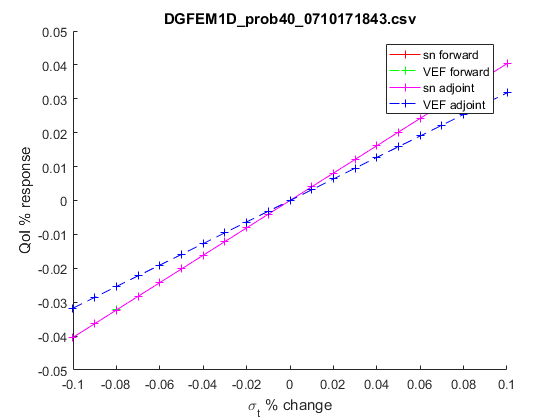
\includegraphics[width=.8\linewidth]{figures/40qSens.png}
  \caption{$\sigt=1$, $\sigs=0.5$}
  \label{fig:sfig2}
\end{subfigure}
\begin{subfigure}{.5\textwidth}
  \centering
  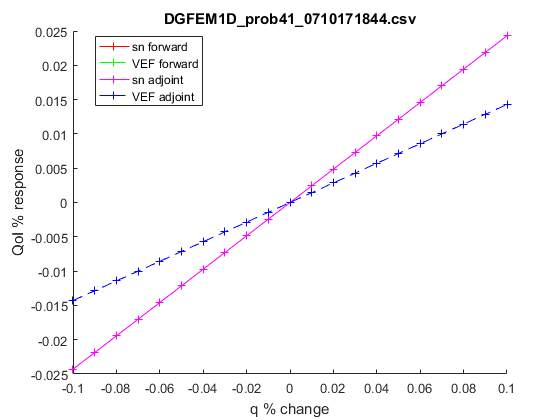
\includegraphics[width=.8\linewidth]{figures/41qSens.png}
  \caption{$\sigt=0.5$, $\sigs=0.25$}
  \label{fig:sfig3}
\end{subfigure}
\caption{Plots of source perturbation sensitivity.}
\label{fig:fig}
\end{figure}

%%%%%%%----------------------------------------------------------------------------------------------
\subsection{Streaming system}
%%%%%%%----------------------------------------------------------------------------------------------

[Formatting graphs]

%%%%%%%%%%%%%%%%%%%%%%%%%%%%%%%%%%%%%%%%%%%%%%%%%%%%%%%%%%%%%%%%%%%%%%%%%%%%%%%%%%%%%%%%%%%%%%%%%%%%%
\section{Goals}
%%%%%%%%%%%%%%%%%%%%%%%%%%%%%%%%%%%%%%%%%%%%%%%%%%%%%%%%%%%%%%%%%%%%%%%%%%%%%%%%%%%%%%%%%%%%%%%%%%%%%

\begin{itemize}
\item Formulate an adjoint equation based on the VET transport formulation, including derivation of appropriate BC for the adjoint unknown.
\item Define the inner products required for first-order sensitivity calculations using the VET formulation for perturbations in cross sections, sources, and incident flux, assuming an unperturbed Eddington Tensor
\item Derive terms that were lost in the first-order adjoint sensitivity formulation due to the assumption that the Eddington remains unperturbed. 
\item Implement the Sn and VET adjoint methods in a 1D FEM solver. 
\item Using 1D test cases, compare the sensitivity values yielded by the VET adjoint method to those obtained by the standard Sn adjoint, as well as sensitivity obtained directly by multiple forward system solves in both Sn and VET.
%\item Consider the alternate boundary conditions presented in Wieselquest. If promise is shown, derive the sensitivity inner products using this boundary condition. Repeat select test cases of the 1D implementation.
\end{itemize}

\newpage

%%%%%%%----------------------------------------------------------------------------------------------
%%%%%%%----------------------------------------------------------------------------------------------
%%%%%%%----------------------------------------------------------------------------------------------
%%%%%%%----------------------------------------------------------------------------------------------
%%%%%%%----------------------------------------------------------------------------------------------
%%%%%%%----------------------------------------------------------------------------------------------
%%%%%%%----------------------------------------------------------------------------------------------
%%%%%%%----------------------------------------------------------------------------------------------
%%%%%%%----------------------------------------------------------------------------------------------

\newpage

%%%%%%
%%%%%%%----------------------------------------------------------------------------------------------

\bibliography{IanProp} 
\bibliographystyle{ieeetr}

%%%%%%%----------------------------------------------------------------------------------------------
\end{document}